%!TEX root = ../Thesis.tex
\chapter{Data}
\section{Sources}
The dataset used in this thesis was constructed from 60 images of raw Linear A inscriptions, and their corresponding ground truth annotations.
\acs{Cefael} \parencite[see][]{EtudesCretoises21} was chosen as the source for raw document images, since it is the only online and widely publicly available source of the printed five volume corpus - \acf{GORILA}. 
As ground truth, annotations provided by Ester Salgarella from SigLA \parencite[see][]{SalgarellaCastellanSigLA2020} were chosen instead of the annotated drawings from the corpus, as the former are more up to date, and of better quality.

What follows in this chapter is a detailed description of this dataset, documenting its characteristics, its construction process, and its limitations and biases.

\section{Characteristics and construction}
The dataset was made to consists of 60 chosen image pairs of raw documents and their corresponding ground truth annotations.
Each of these image pairs was categorized into one of three difficulty levels (easy, medium, hard) based on the visual quality of the inscriptions (see \cref{sec:difficulty_classification}).
They were then split into a test set of 27 images, a validation set of 27 images, and a support set of 6 images, with each set containing an equal proportion of images from each of the three difficulty levels.

Only inscriptions with clay as writing support were included, as they are the most common and representative of the Linear A corpus, and were the only ones for which SigLA ground truth annotations were already available.
The raw document images from \acs{Cefael} are screenshots of grayscale images placed within the scanned printed edition of the corpus, and are thus not of the highest quality, being the only widely publicly available images of the Linear A inscriptions.
For an example of a raw document image and its corresponding ground truth annotation, see Figure \ref{fig:ht7b_example}.
\begin{figure}[htbp]
\centering
\begin{subfigure}[t]{0.4\textwidth}
    \centering
    \fbox{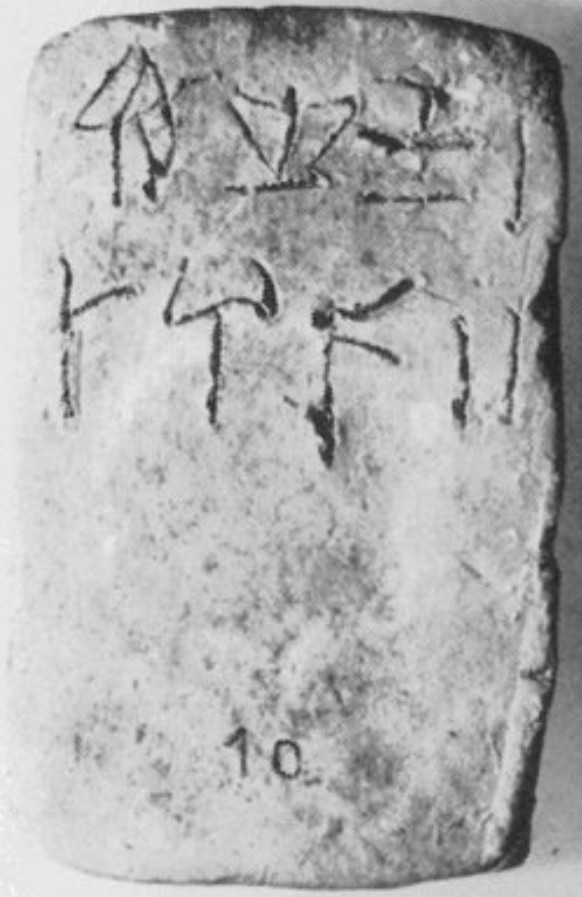
\includegraphics[width=\linewidth]{../src/data/raw/easy/HT7b.jpg}}
    \caption{Raw image (HT7b)}
\end{subfigure}
\hspace{0.04\textwidth}
\begin{subfigure}[t]{0.4\textwidth}
    \centering
    \fbox{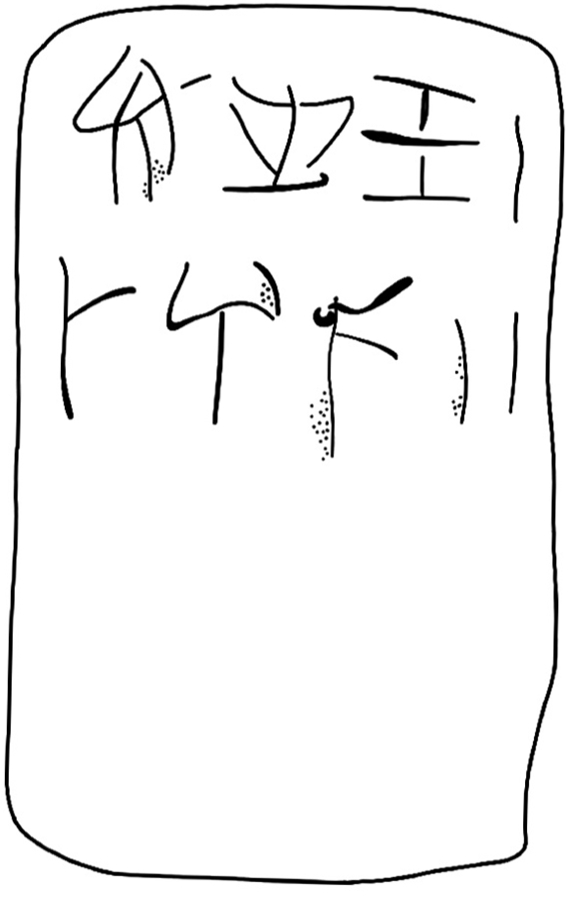
\includegraphics[width=\linewidth]{../src/data/ground_truth/registered/HT7b.jpg}}
    \caption{Ground truth (HT7b)}
\end{subfigure}

\caption{Example of a raw inscription image and its corresponding ground truth annotation.}
\label{fig:ht7b_example}
\end{figure}

\subsection{Difficulty classification}
\label{sec:difficulty_classification}
The dataset was categorized into three difficulty levels (easy, medium, hard) based on the visual quality of the raw images and the clarity of the inscriptions.
This classification was performed manually by inspecting each image and considering factors such as contrast, noise, and the presence of tablet breakages or general damage to the inscriptions.
The concrete criteria used to classify the difficulty sets were as follows:
\begin{itemize}
    \item \textbf{Easy:} labeled as such for documents with clear ingravings, good contrast, minimal noise, and constant lighting.
    \item \textbf{Hard:} labeled to those with poor contrast, significant noise, and substantial damage making it hard even for the naked eye to read the inscriptions.
    \item \textbf{Medium:} labeled to all those inbetween the qualities of easy and hard.
\end{itemize}
For visual examples of images within each of these difficulties, see \cref{fig:difficulty_examples}.


\begin{figure}[htbp]
\centering

\begin{subfigure}[c]{0.45\textwidth}
    \centering
    \fbox{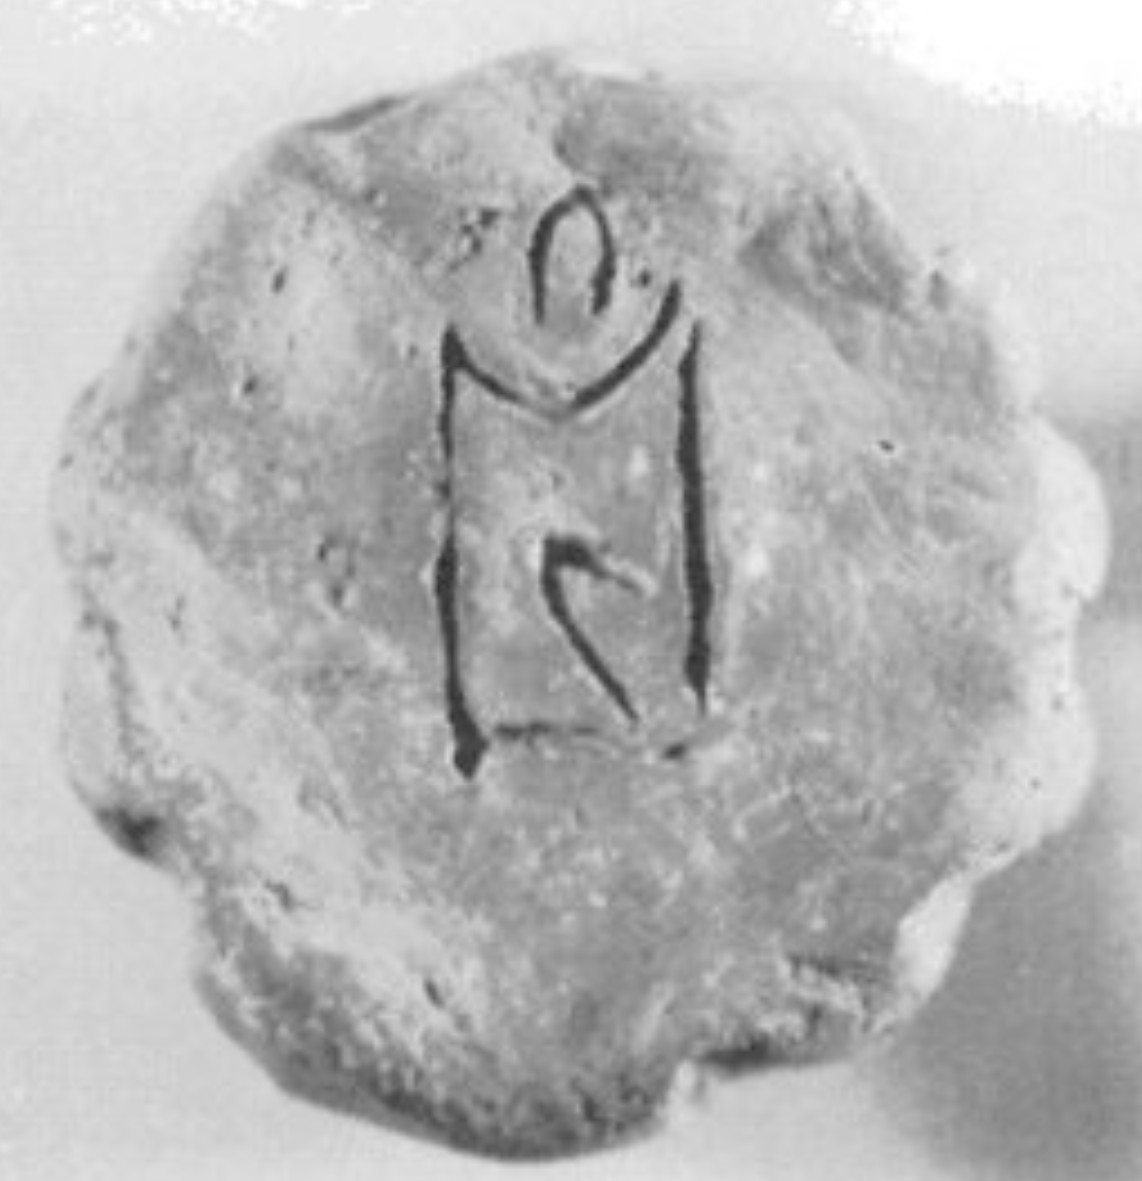
\includegraphics[width=\linewidth]{../src/data/raw/easy/KHWc2104.jpg}}
    \caption{Easy KHWc2104 (raw)}
\end{subfigure}
\hspace{0.02\textwidth}
\begin{subfigure}[c]{0.45\textwidth}
    \centering
    \fbox{
\includegraphics[width=\linewidth]{../src/data/ground_truth/registered/KHWc2104.jpg}}
    \caption{Easy KHWc2104 (gt)}
\end{subfigure}

\vspace{0.6em}

\begin{subfigure}[c]{0.45\textwidth}
    \centering
    \fbox{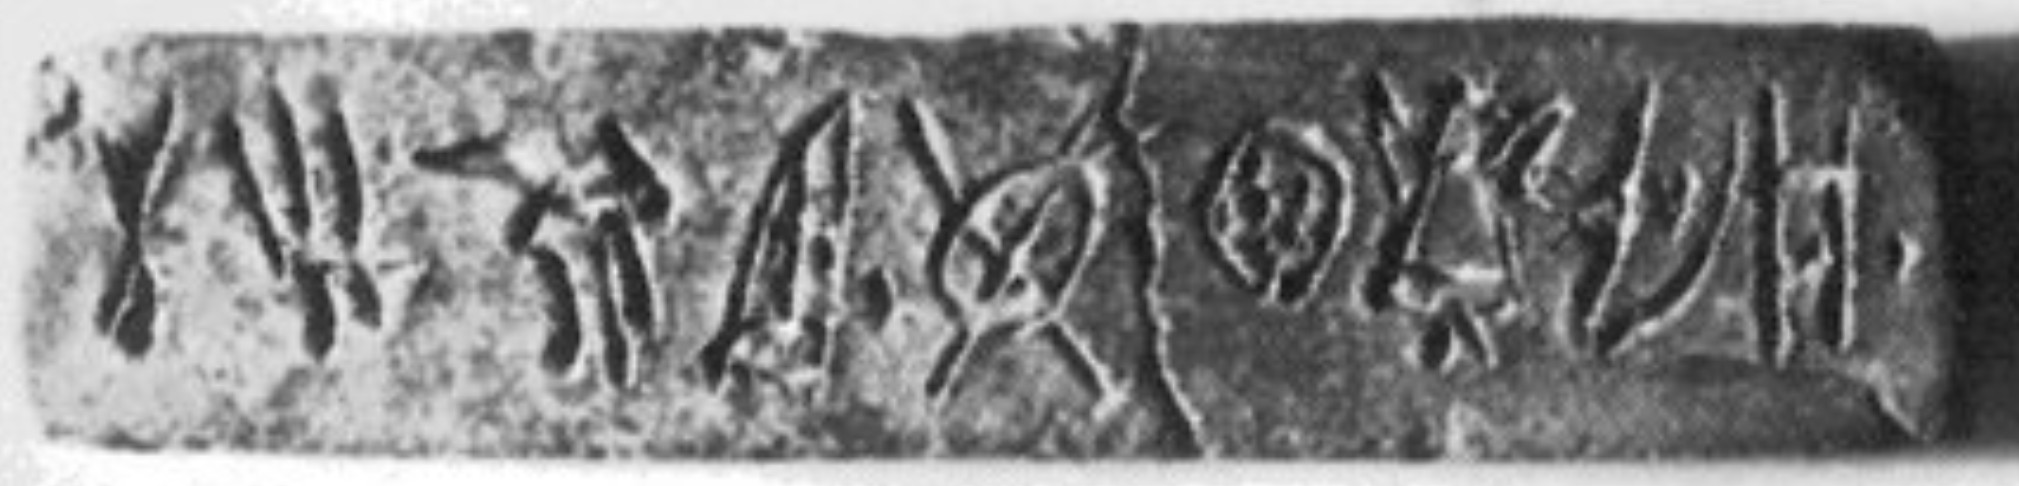
\includegraphics[width=\linewidth]{../src/data/raw/medium/MA1a.jpg}}
    \caption{Medium MA1a (raw)}
\end{subfigure}
\hspace{0.02\textwidth}
\begin{subfigure}[c]{0.45\textwidth}
    \centering
    \fbox{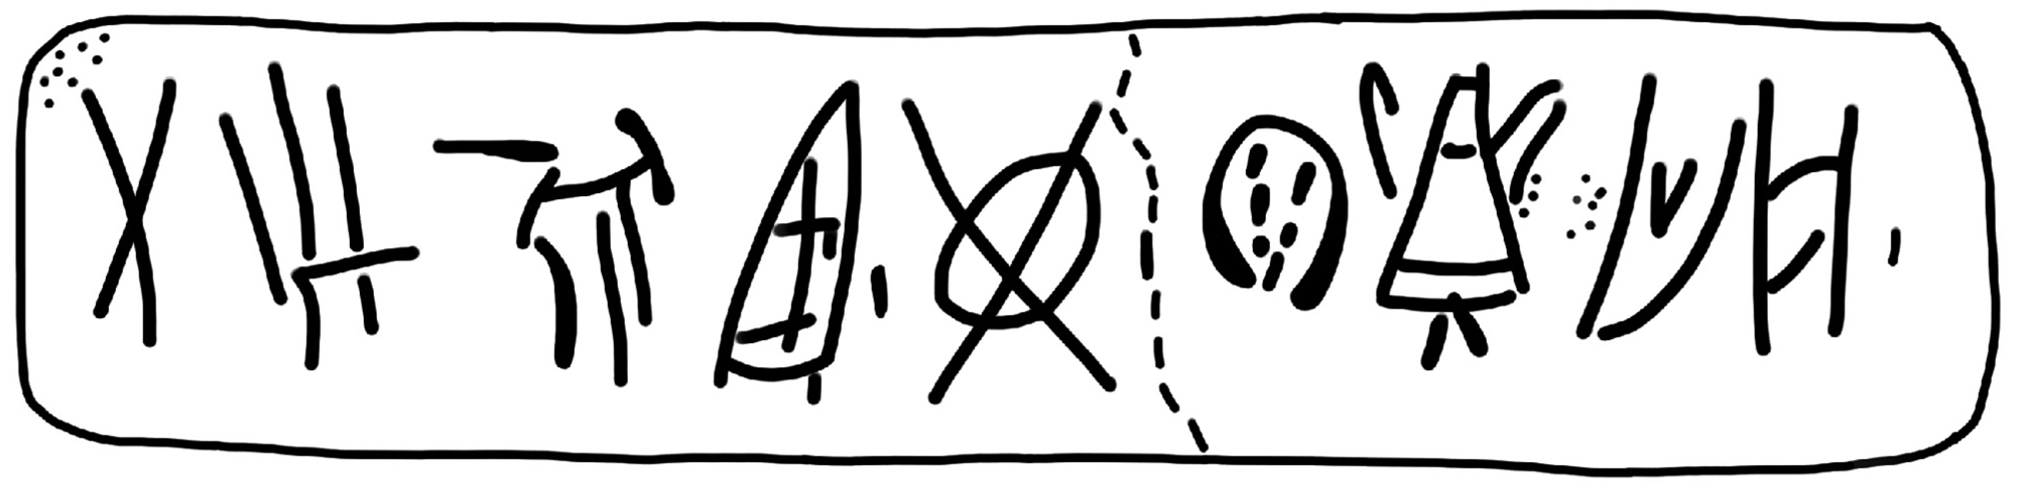
\includegraphics[width=\linewidth]{../src/data/ground_truth/registered/MA1a.jpg}}
    \caption{Medium MA1a (gt)}
\end{subfigure}

\vspace{0.6em}

\begin{subfigure}[c]{0.45\textwidth}
    \centering
    \fbox{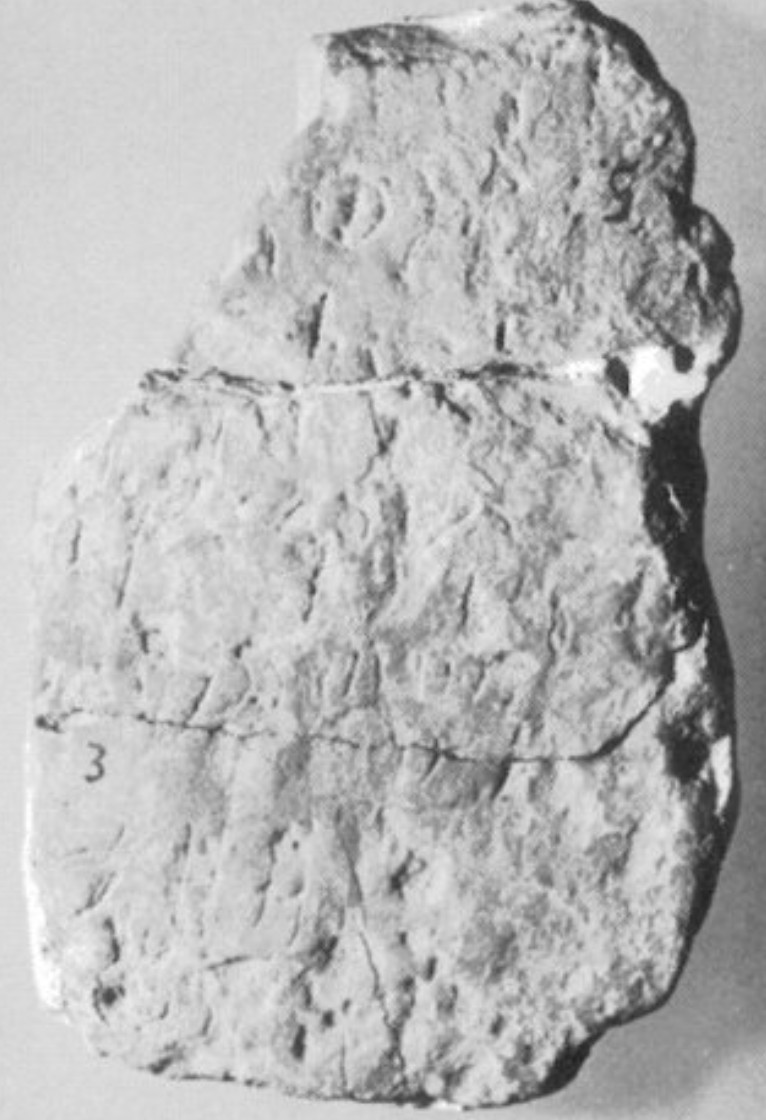
\includegraphics[width=\linewidth]{../src/data/raw/hard/HT3.jpg}}
    \caption{Hard HT3 (raw)}
\end{subfigure}
\hspace{0.02\textwidth}
\begin{subfigure}[c]{0.45\textwidth}
    \centering
    \fbox{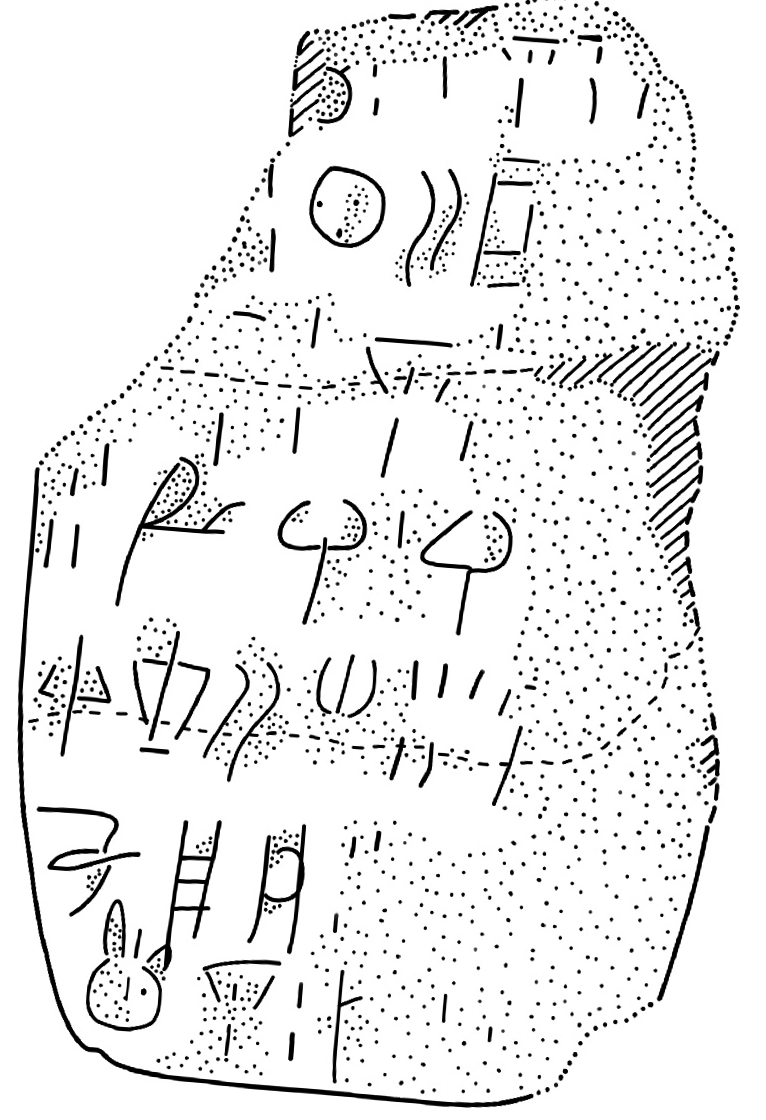
\includegraphics[width=\linewidth]{../src/data/ground_truth/registered/HT3.jpg}}
    \caption{Hard HT3 (ground truth)}
\end{subfigure}

\caption{Examples of images with different levels of segmentation difficulty: easy, medium, and hard. For each case, the raw image (left) and the corresponding ground truth annotation (right) are shown.}
\label{fig:difficulty_examples}

\end{figure}

\subsection{Image registration and preprocessing}
To obtain any kind of meaningful comparison between model outputs and ground truth, the raw images and their ground truth annotations had to be aligned and registered to each other.
This was done manually in Krita for all 60 image pairs by downscaling the ground truth images to the individual scales of their raw counterparts, and aligning by translation and rotation, using the raw images as background reference.


\section{Limitations and biases}
\subsection{Quality of the raw tablet images}
Due to the weak quality of the raw tablet images, they carry only parts of the visual information of the tablets they represent.
When the drawings of \acs{GORILA} were made, the researchers had access to the tablets themselves, meaning they could see what the images did not pick up, and better discern actual engravings from mere damages to the tablets. 
Therefore, these tablet images are far from the best source of data there is, being however, the only source publicly available.
That lack of good quality data can unfortunately limits the output quality of segmentations constructed therefrom.
\subsection{Alignment to the ground truth}
Even after image registration, ground truth images still did not perfectly align with the raw images, affecting the obtained segmentation quality.
This misalignment was a source of noise in the evaluation.
Ester's annotations were never constructed by overlaying them on the raw images, but rather by doing so on the accompanied corpus drawings, only using the raw images as reference.
Thus, the raw images and the ground truth annotations were never perfectly aligned to begin with, and the manual registration process could only do so much to mitigate that.
This is seen by the low \acs{Dice} values obtained for all models in the results (see \cref{rq1results}).

\subsection{Binarization of the drawings}
Due to a missing threshold step of the registered JPEGs in the initial registration of the dataset, the ground truth annotations were to begin with binarized with a threshold of 0 instead of 128, meaning that only the pure black pixels of the drawings were considered as part of the ground truth foreground, while the lighter gray pixels were not accounted for.
This led to lower \acs{Dice} scores in general, as the ground truth in practice was thinner and more sparse compared to the actual drawings.

This issue was for the evaluation later corrected to a threshold of 128, meaning that all pixels darker than 128 now were considered foreground, and all pixels lighter than that were considered background (see \cref{fig:binarization_examples} for visual examples of the two different ways of binarization).
However, only the hyperparameter optimization of the models was not redone for the new binarization format, and was thus performed with ground truth in the old binarization format.

Arguably, this only affected the effectiveness of the optimization and what the models were optimized for (penalizing non-conservative segmentation styles  more than otherwise), while still preserving fairness and generalizability, as all model hyperparameters were tuned under the same conditions.
 
\begin{figure}[htbp]
\centering

\begin{subfigure}[c]{0.45\textwidth}
    \centering
    \fbox{
\includegraphics[width=\linewidth]{../src/data/ground_truth/registered0/KHWc2104.png}}
    \caption{KHWc2104 (old)}
\end{subfigure}
\hspace{0.02\textwidth}
\begin{subfigure}[c]{0.45\textwidth}
    \centering
    \fbox{
\includegraphics[width=\linewidth]{../src/data/ground_truth/registered2/KHWc2104.png}}
    \caption{KHWc2104 (new)}
\end{subfigure}

\vspace{0.6em}

\begin{subfigure}[c]{0.45\textwidth}
    \centering
    \fbox{
\includegraphics[width=\linewidth]{../src/data/ground_truth/registered0/MA1a.png}}
    \caption{MA1a (old)}
\end{subfigure}
\hspace{0.02\textwidth}
\begin{subfigure}[c]{0.45\textwidth}
    \centering
    \fbox{
\includegraphics[width=\linewidth]{../src/data/ground_truth/registered2/MA1a.png}}
    \caption{MA1a (new)}
\end{subfigure}

\vspace{0.6em}

\begin{subfigure}[c]{0.45\textwidth}
    \centering
    \fbox{
\includegraphics[width=\linewidth]{../src/data/ground_truth/registered0/HT3.png}}
    \caption{HT3 (old)}
\end{subfigure}
\hspace{0.02\textwidth}
\begin{subfigure}[c]{0.45\textwidth}
    \centering
    \fbox{
\includegraphics[width=\linewidth]{../src/data/ground_truth/registered2/HT3.png}}
    \caption{HT3 (new)}
\end{subfigure}

\caption{Examples of images processed with the two different binarization thresholds; 0 (old) and 128 (new).}
\label{fig:binarization_examples}

\end{figure}